%===========================================
\documentclass[12pt]{article}
%===========================================
\usepackage[latin1]{inputenc}
%\usepackage[margin=2.5in]{geometry}
\usepackage{amsmath,amssymb,amsthm,amsfonts}
\usepackage{hyperref}
\usepackage[spanish]{babel}
\usepackage{fancyhdr}
\usepackage{titlesec}
\usepackage{listings}
\usepackage{graphicx,graphics}
\usepackage{multicol}
\usepackage{multirow}
\usepackage{color}
\usepackage{float} 
\usepackage{subfig}
\usepackage[figuresright]{rotating}
\usepackage{enumerate}
\usepackage{anysize} 
\usepackage{url}
\usepackage{imakeidx}
\usepackage[left=0.5in, right=0.5in, top=1in, bottom=1in]{geometry}
% Opcional: para incluir gráficos con control de tamaño
\usepackage{float}

\hyphenation{mo-de-ra-da-men-te}
\addto\captionsspanish{\renewcommand{\figurename}{Figura}}

%===========================================
% Ajustes de Sweave
%\usepackage{Sweave}
%===========================================
\title{Notas sobre Métodos Numéricos con R}
\author{
Carlos E. Martínez-Rodríguez \\
Universidad Autónoma de la Ciudad de México \\
Academia de Matemáticas \\
\texttt{carlos.martinez@uacm.edu.mx}
}
\date{Agosto 2025}
\date{}
%===========================================
\newtheorem{Criterio}{Criterio}%[section]
\newtheorem{Sup}{Supuesto}%[section]
\newtheorem{Note}{Nota}%[section]
\newtheorem{Ejem}{Ejemplo}%[section]
\newtheorem{Prop}{Proposici\'on}%[section]
\newtheorem{Def}{Definici\'on}
\newtheorem{Teo}{Teorema}
\newtheorem{Algthm}{Algoritmo}
\newtheorem{Sol}{Soluci\'on}
%===========================================
\begin{document}
\maketitle
\tableofcontents

%===========================================
\section{Sobre el curso}
%===========================================

El curso se llevará a cabo tres veces a la semana,  con sesiones de 1.5 horas,  de las cuales una de ellas se realizará en el laboratorio de cómputo 3.

%---------------------------------------------------
\subsection{Requisitos para acreditar la materia}
%---------------------------------------------------

El curso por su naturaleza implica que la/el estudiante implemente los distintos algoritmos que se revisan en el curso,  por lo tanto es importante que demuestre que efectivamente puede implementar, revisar y mejorar los algoritmos ya existentes.\bigskip

Hay dos maneras de certificar la materia: a) Portafolio y b) Examen de certificación.  Al menos una semana antes de que termine el curso las y los estudiantes tendrán conocimiento de sus calificaciones parciales y por tanto de la calificación promedio obtenida al momento, para que sea el/la mismo(a) estudiante quién decida si certifica por la modalidad de portafolio,  o por la modalidad de examen de certificación.\bigskip


El portafolio se conforma de evaluaciones ($40\%$), programas, ($40\%$) tareas ($10\%$), tareitas ($5\%$)y trabajos adicionales ($5\%$). Mientras que la certificación es un examen elaborado por el comité de certificación y que será presentado por todas y todos los estudiantes que se inscriban en esta modalidad en las fechas establecidas por la Coordinación de Certificación y Registro.  En cualquiera de las dos modalidades es indispensable que el/la estudiante se registre a este proceso para que su calificación pueda ser asignada al final del proceso de Certificación.

%---------------------------------------------------
\subsection{De la naturaleza del curso}
%---------------------------------------------------

El curso tiene un fuerte sustento en la programación constante, sin embargo, es importante resaltar que los conceptos teóricos deben ser dominados por las y los estudiantes, por lo tanto las evaluaciones y las tareas tendrán estas dos componentes principales.  Al contrario de lo que pueda pensarse la asistencia al curso es obligatoria pero no influye directamente en la calificación obtenida.  Sin embargo,  hay que mencionar que si la asistencia se realiza de manera intermitente es probable que cueste un poco de trabajo reincorporarse a la dinámica de trabajo que se irá construyendo con el grupo con el transcurso de las clases. 

%===========================================
\section{Introducción}
%===========================================

En este curso estudiaremos los elementos básicos de los métodos numéricos, utilizando el programa de distribución libre \textit{R}. Antes de iniciar propiamente con el estudio de los métodos numéricos realizaremos un breve repaso de algunos conceptos de álgebra lineal, cálculo diferencial mismos que son fundamentales en esta materia y de la que se supone las y los estudiantes se encuentran familiarizados con ellos.

%===========================================
\section{Revisión de temas importantes}
%===========================================

%-------------------------------------------
\subsection{Cálculo}
%-------------------------------------------

Comenzamos el capítulo con un repaso de algunos aspectos importantes del cálculo que son necesarios a lo largo del texto. Suponemos que los estudiantes que lean este texto conocen la terminología, la notación y los resultados que se dan en un curso típico de cálculo.

%...............................................................
\subsubsection{Límites y continuidad}
%...............................................................

El límite de una función nos dice qué tan cerca se encuentran las imágenes de una función si dos elementos de su dominio se encuentran lo suficientemente cerca, es decir, decimos que una función $f(x)$ definida en el intervalo $(a,b)$ tiene \textbf{límite} $L$ en el punto $x = x_0$, lo que denotamos por $$\lim_{x \to x_0} f(x) = L,$$ si para cualquier $\varepsilon > 0$, existe un número real $\delta > 0$ tal que $|f(x) - L| < \varepsilon$ siempre que $0 < |x - x_0| < \delta $. Es decir, que los valores de la función estarán cerca de $L$ siempre que $x$ esté suficientemente cerca de $x_0$.
\bigskip

Se dice que una función $f$ es continua en $a$ si cuando $x$ se aproxima al valor de $a$, entonces también $f(x)$ se aproxima a $f(a)$, es decir, $f(x)$ es \textbf{continua} en el punto $x = a $ si $$\lim_{x \to a} f(x) = f(a),$$
y se dice que $f$ es \textbf{continua en el conjunto} $(a,b)$ si es continua en cada uno de los puntos del intervalo. Denotaremos el conjunto de todas las funciones $f$ que son continuas en $E=(a,b)$ por $C(E)$. \bigskip

Se dice que una sucesión $\{x_n\}_{n=1}^\infty$ \textbf{converge} a un número $x$, si
$\lim_{n \to \infty} x_n = x$ o bien, $x_n \to x$ cuando $n \to \infty$, si para cualquier $\varepsilon > 0$, existe un número natural $N(\varepsilon)$ tal que $|x_n - x| < \varepsilon$ para cada $n > N(\varepsilon)$. Cuando una sucesión tiene límite, se dice que la \textbf{sucesión converge}.

%........................................................
\subsubsection{Continuidad y convergencia de sucesiones}
%........................................................

Si $f(x)$ es una función definida en un conjunto $S$ de números reales y $x_0 \in S$, entonces las siguientes afirmaciones son equivalentes:
\begin{enumerate}
\item $f(x) $ es continua en $x = x_0 $,
\item Si $\{x_n\}_{n=1}^\infty $ es cualquier sucesión en $S $ que converge a $x_0 $, entonces $\lim_{n \to \infty} f(x_n) = f(x_0).$
\end{enumerate}

\begin{Teo}[Teorema del valor intermedio o de Bolzano.]
Si $f \in C[a, b] $ y $\ell $ es un número cualquiera entre $f(a) $ y $f(b) $, entonces existe al menos un número $c \in (a, b) $ tal que $f(c) = \ell $. Véase la Figura~\ref{fig:bolzano}.

\begin{figure}[H]
\centering
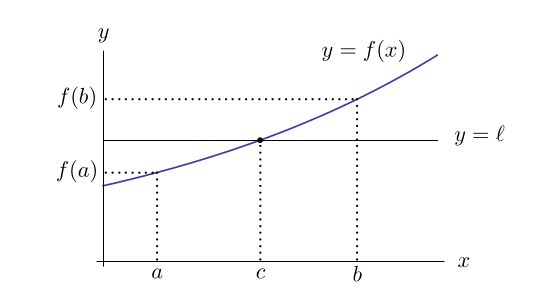
\includegraphics[width=0.65\textwidth]{Fig1.png}
\caption{Teorema del valor intermedio o de Bolzano}
\label{fig:bolzano}
\end{figure}
\end{Teo}


\begin{Note}
Todas las funciones con las que se van a trabajar en este curso de métodos numéricos serán continuas, ya que esto es lo mínimo que debemos exigir para asegurar que la conducta de un método se puede predecir.
\end{Note}

%........................................................
\subsubsection{Derivabilidad}
%........................................................

Si $f(x) $ es una función definida en un intervalo abierto que contiene un punto $x_0 $, entonces se dice que $f(x) $ es \textbf{derivable} en $x = x_0 $ cuando existe el límite
$$f'(x_0) = \lim_{x \to x_0} \frac{f(x) - f(x_0)}{x - x_0}.$$

El número $f'(x_0)$ se llama \textbf{derivada} de $f$ en $x_0$ y coincide con la pendiente de la recta tangente a la gráfica de $f$ en el punto $(x_0, f(x_0))$, Figura~\ref{fig:derivada}.

\begin{figure}[H]
\centering
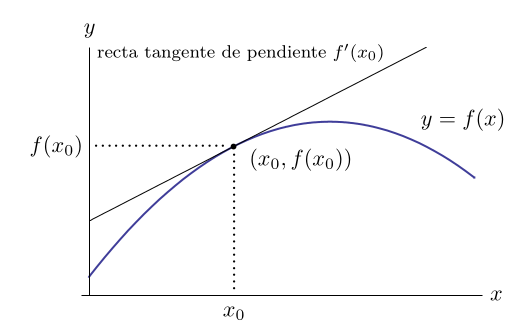
\includegraphics[width=0.65\textwidth]{Fig2.png}
\caption{Derivada de una función en un punto}
\label{fig:derivada}
\end{figure}

\textbf{Derivabilidad implica continuidad.} Si la función $f(x)$ es derivable en $x = x_0$, entonces $f(x)$ es continua en $x = x_0$. El conjunto de todas las funciones que admiten $n$ derivadas continuas en $S $ se denota por $C^n(S)$, mientras que el conjunto de todas las funciones indefinidamente derivables en $S$ se denota por $C^\infty(S)$. Las funciones polinómicas, racionales, trigonométricas, exponenciales y logarítmicas están en $C^\infty(S)$, siendo $S$ el conjunto de puntos en los que están definidas.

\begin{Teo}[Teorema del valor medio o de Lagrange.]
Si $f\in C[a, b]$ y es derivable en $(a,b)$, entonces existe un punto $c\in (a,b)$ tal que
$$f'(c) = \frac{f(b) - f(a)}{b - a}.$$
\end{Teo}

Geométricamente hablando, Figura~\ref{fig:lagrange}, el teorema del valor medio dice que hay al menos un número $c \in (a, b) $ tal que la pendiente de la recta tangente a la curva $y = f(x) $ en el punto $(c, f(c)) $ es igual a la pendiente de la recta secante que pasa por los puntos $(a, f(a)) $ y $(b, f(b)) $.

\begin{figure}[H]
\centering
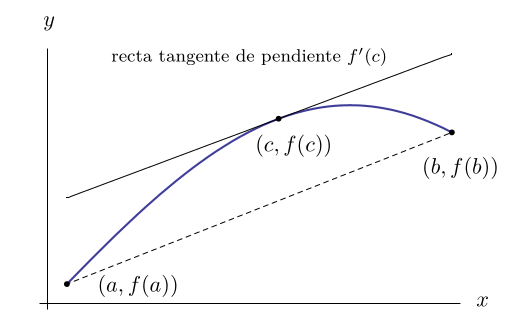
\includegraphics[width=0.65\textwidth]{Fig3.png}
\caption{Teorema del valor medio o de Lagrange}
\label{fig:lagrange}
\end{figure}

\begin{Teo}[Teorema de los valores extremos.]  
Si $f \in C[a,b] $, entonces existen $c_1 $ y $c_2 $ en $(a,b) $ tales que $f(c_1) \leq f(x) \leq f(c_2) $ para todo $x \in [a,b] $. Si además, $f $ es derivable en $(a,b) $, entonces los puntos $c_1 $ y $c_2 $ están en los extremos de $[a,b] $ o bien son puntos críticos.
\end{Teo}

%........................................................
\subsubsection{Integración}
%........................................................


\begin{Teo}[Primer teorema fundamental o regla de Barrow.]
  Si $f \in C[a, b] $ y $F $ es una primitiva cualquiera de $f $ en $[a, b] $ (es decir, $F'(x) = f(x) $), entonces $$\int_a^b f(x) \, dx = F(b) - F(a). $$
\end{Teo}

\begin{Teo}[Segundo teorema fundamental.]
  Si $f \in C[a, b] $ y $x \in (a, b) $, entonces $$\frac{d}{dx} \int_a^x f(t) \, dt = f(x).$$
\end{Teo}

\begin{Teo}[Teorema del valor medio para integrales.]
  Si $f \in C[a, b] $, $g $ es integrable en $[a, b] $ y $g(x) $ no cambia de signo en $[a, b] $, entonces existe un punto $c \in (a, b) $ tal que  $$\int_a^b f(x)g(x) \, dx = f(c) \int_a^b g(x) \, dx.$$
\end{Teo}

\begin{Note}
Cuando $g(x) = 1 $, véase la Figura~\ref{fig:valormedio-integral}, este resultado es el habitual teorema del valor medio para integrales y proporciona el valor medio de la función $f $ en el intervalo $[a, b] $, que está dado por $$f(c) = \frac{1}{b-a} \int_a^b f(x) \, dx.$$

\begin{figure}[H]
\centering
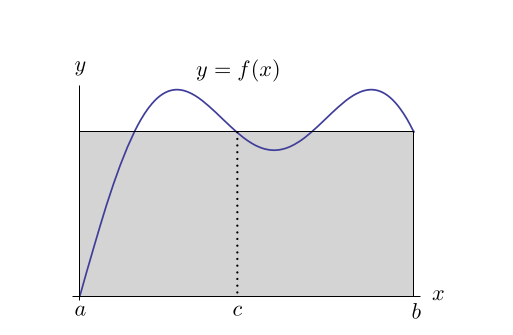
\includegraphics[width=0.65\textwidth]{Fig4.png}
\caption{Teorema del valor medio para integrales}
\label{fig:valormedio-integral}
\end{figure}
\end{Note}

%...............................................................
\subsubsection{Polinomios de Taylor}
%...............................................................

\begin{Teo}[Teorema de Taylor.]
Supongamos que $f \in C^{(n)}[a,b] $ y que $f^{(n+1)} $ existe en $[a,b] $. Sea $x_0 $ un punto en $[a,b] $. Entonces, para cada $x $ en $[a,b] $, existe un punto $\xi(x) $ entre $x_0 $ y $x $ tal que
$$f(x) = P_n(x) + R_n(x),$$
donde
\begin{eqnarray}
P_n(x) &=& f(x_0) + f'(x_0)h + \frac{f''(x_0)}{2!}h^2 + \cdots + \frac{f^{(n)}(x_0)}{n!}h^n = \sum_{k=0}^n \frac{f^{(k)}(x_0)}{k!} h^k,\\
R_n(x)&=& \frac{f^{(n+1)}(\xi(x))}{(n+1)!} h^{n+1}, \quad \text{y} \quad h = x - x_0.
\end{eqnarray}
\end{Teo}


El polinomio $P_n(x) $ se llama \textbf{n-ésimo polinomio de Taylor} de $f $ alrededor de $x_0 $ (véase la Figura~\ref{fig:taylor}).   $R_n(x) $ se llama \textbf{error de truncamiento} (o \textit{resto de Taylor}) asociado a $P_n(x) $.   Como el punto $\xi(x) $ en el error de truncamiento $R_n(x) $ depende del punto $x $ en el que se evalúa el polinomio $P_n(x) $, podemos verlo como una función de la variable $x $.

\begin{figure}[H]
\centering
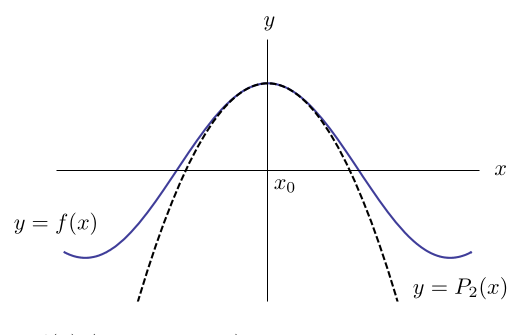
\includegraphics[width=0.6\textwidth]{Fig5.png}
\caption{Gráficas de $y = f(x) $ y de su polinomio de Taylor $y = P_2(x) $ alrededor de $x_0 $.}
\label{fig:taylor}
\end{figure}

\begin{Note}
La serie infinita que resulta al tomar límite en la expresión de $P_n(x) $ cuando $n \to \infty $ se llama \textbf{serie de Taylor} de $f $ alrededor de $x_0 $. Cuando $x_0 = 0 $, el polinomio de Taylor se suele denominar \textbf{polinomio de Maclaurin}, y la serie de Taylor se llama \textbf{serie de Maclaurin}.\bigskip

La denominación \textit{error de truncamiento} en el teorema de Taylor se refiere al error que se comete al usar una suma truncada al aproximar la suma de una serie infinita.
\end{Note}

%...............................................................
\subsubsection{Teoremas adicionales}
%...............................................................

A continuación enunciaremos algunas de las definiciones y teoremas básicos que utilizaremos a lo largo de estas notas.

\begin{Def}$f$ es de clase $C^1$ en el intervalo $[a;b]$ si $f'$ es continua en $[a;b]$.
\end{Def}

\begin{Def}$f$ es de clase $C^n$ en el intervalo $[a;b]$ si $f^{(n)}$ es continua en $[a;b]$.
\end{Def}

\begin{Def}$f$ es de clase $C^\infty$ en el intervalo $I$ si $f$ es infinitas veces derivable y continua en $I$.
\end{Def}

\begin{Teo} (Teorema de los valores intermedios). Sea $f$ continua en el intervalo $[a;b]$. Si $k \in \mathbb{R}$ es un número comprendido entre $f(a)$ y $f(b)$, entonces existe al menos un punto $\xi$ perteneciente al intervalo $(a;b)$ tal que $f(\xi) = k$.
\end{Teo}

\begin{Teo}[Bolzano]Si $f$ es continua en el intervalo $[a;b]$ y $f(a) \cdot f(b) < 0$, entonces existe un $\xi$ perteneciente al $(a;b)$ tal que $f(\xi) = 0$.
\end{Teo}

\begin{Teo}[Teorema de acotabilidad] Si $f : [a;b] \mapsto \mathbb{R}$ es continua en $[a;b]$, entonces $f$ está acotada en $[a;b]$.
\end{Teo}

\begin{Teo}[Teorema de Weierstrass] Si $f : [a;b] \mapsto \mathbb{R}$ es continua en $[a;b]$, entonces $f$ tiene un máximo global y un mínimo global en $[a;b]$.
\end{Teo}

\begin{Teo}[Teorema Generalizado de Rolle] Si $f$ continua en $[a;b]$, y existen las derivadas $f'(x), f''(x), \ldots, f^{(n)}(x)$ en $(a;b)$ y $f(x_0) = f(x_1) = \cdots = f(x_n) = 0$ (con $x_0, x_1, \ldots, x_n \in [a;b]$) entonces existe $\xi$ perteneciente al $(a;b)$ tal que $f^{(n)}(\xi) = 0$.
\end{Teo}

\begin{Teo}[Teorema de Lagrange] Si $f$ continua en $[a;b]$ y derivable en $(a;b)$ entonces existe $\xi$ perteneciente al $(a;b)$ tal que $f(b) - f(a) = f'(\xi)(b - a)$.
\end{Teo}

\begin{Teo}[Teorema del valor medio ponderado] Sea $f$ continua en $[a,b]$ y $g$ una función integrable Riemann en $[a,b]$. Si $g$ no cambia de signo en $[a,b]$, entonces existe un número $c \in (a,b)$ tal que:
$$\int_a^b f(x)g(x)dx = f(c) \int_a^b g(x)dx$$
\end{Teo}

%-------------------------------------------
\subsection{Álgebra Lineal}
%-------------------------------------------

%...............................................................
\subsubsection{Matrices}
%...............................................................

Una \textbf{matriz} es un arreglo multidimensional de escalares, llamados \textit{elementos}, ordenados en filas y columnas.  Una matriz de $ m $ filas y $ n $ columnas, o \textit{matriz (de orden) $ m \times n $}, es un conjunto de $ m \cdot n $ elementos $ a_{ij} $, con $ i = 1, 2, \ldots, m $ y $ j = 1, 2, \ldots, n $, que se representa de la siguiente forma:
$$A = \begin{pmatrix}
a_{11} & a_{12} & \cdots & a_{1n} \\
a_{21} & a_{22} & \cdots & a_{2n} \\
\vdots & \vdots & \ddots & \vdots \\
a_{m1} & a_{m2} & \cdots & a_{mn}
\end{pmatrix}$$

Se puede abreviar la representación de la matriz anterior de la forma $ A = (a_{ij}) $ con $ i = 1, 2, \ldots, m $; $ j = 1, 2, \ldots, n $.

Hay una relación directa entre matrices y vectores puesto que podemos pensar una matriz como una composición de vectores fila o de vectores columna. Además, un vector es un caso especial de matriz: un \textit{vector fila} es una matriz con una sola fila y varias columnas, y un \textit{vector columna} es una matriz con varias filas y una sola columna. 

%...............................................................
\subsubsection{Operaciones con matrices}
%...............................................................

\begin{itemize}
\item Si $ A = (a_{ij}) $ y $ B = (b_{ij}) $ son dos matrices que tienen el mismo orden, $ m \times n $, decimos que $ A $ y $ B $ son \textbf{iguales} si $ a_{ij} = b_{ij} $ para todo $ i = 1, \ldots, m $ y $ j = 1, \ldots, n $.

\item Si $ A = (a_{ij}) $ y $ B = (b_{ij}) $ son dos matrices que tienen el mismo orden $ m \times n $, la \textbf{suma} de $ A $ y $ B $ es una matriz $ C = (c_{ij}) $ del mismo orden con $ c_{ij} = a_{ij} + b_{ij} $ para todo $ i = 1, \ldots, m $ y $ j = 1, \ldots, n $.

\item Si $ A = (a_{ij}) $ es una matriz de orden $ m \times n $, la \textbf{multiplicación de $ A $ por un escalar} $ \lambda $ es una matriz $ C = (c_{ij}) $ del mismo orden $ m \times n $ con $ c_{ij} = \lambda a_{ij} $ para todo $ i = 1, \ldots, m $ y $ j = 1, \ldots, n $.

\item Si $ A = (a_{ij}) $ es una matriz de orden $ m \times n $, la \textbf{matriz traspuesta} de $ A $ es la matriz que resulta de intercambiar sus filas por sus columnas, se denota por $ A^T $ y es de orden $ n \times m $.

\item Si $ A = (a_{ij}) $ es una matriz de orden $ m \times p $ y $ B = (b_{ij}) $ es una matriz de orden $ p \times n $, el \textbf{producto de $ A $ por $ B $} es una matriz $ C = (c_{ij}) $ de orden $ m \times n $ con $$c_{ij} = \sum_{k=1}^p a_{ik}b_{kj}, \quad \text{para todo } i = 1, \ldots, m \text{ y } j = 1, \ldots, n.$$ Obsérvese que el producto de dos matrices solo está definido si el número de columnas de la primera matriz coincide con el número de filas de la segunda.
\end{itemize}

%...............................................................
\subsubsection{Matrices especiales}
%...............................................................
\begin{itemize}

\item Una matriz $ A = (a_{ij}) $ es \textbf{cuadrada} si tiene el mismo número de filas que de columnas, y de orden $ n $ si tiene $ n $ filas y $ n $ columnas. Se llama \textbf{diagonal principal} al conjunto de elementos $ a_{11}, a_{22}, \ldots, a_{nn} $.

\item Una \textbf{matriz diagonal} es una matriz cuadrada que tiene algún elemento distinto de cero en la diagonal principal y ceros en el resto de elementos.

\item Una matriz cuadrada con ceros en todos los elementos por encima (debajo) de la diagonal principal se llama \textbf{matriz triangular inferior (superior)}.

\item Una matriz diagonal con unos en la diagonal principal se denomina \textbf{matriz identidad} y se denota por $I$. Es la única matriz cuadrada tal que $ AI = IA = A $ para cualquier matriz cuadrada $A$.

\item Una \textbf{matriz simétrica} es una matriz cuadrada $A$ tal que $A=A^T$.

\item La \textbf{matriz cero} es una matriz con todos sus elementos iguales a cero.

\item Decimos que una matriz cuadrada $A$ es \textbf{invertible} (o \textit{regular} o \textit{no singular}) si existe una matriz cuadrada $ B $ tal que $AB = BA = I$. Se dice entonces que $ B $ es la \textbf{matriz inversa} de $A$ y se denota por $A^{-1}$. (Una matriz que no es invertible se dice \textit{singular}.)

\item Si una matriz $ A $ es invertible, su inversa también lo es y $A^{-1})^{-1} = A$.

\item Si $A$ y $B$ son dos matrices invertibles, su producto también lo es y $(AB)^{-1} = B^{-1}A^{-1}$.
\end{itemize}


%...............................................................
\subsubsection{Determinante de una matriz}
%...............................................................

El \textbf{determinante} de una matriz solo está definido para matrices cuadradas y su valor es un escalar.  El determinante de una matriz $ A $ cuadrada de orden $ n $ se denota por $ |A| $ o $ \det(A) $, y se define como
$$\det(A) = \sum_{j} (-1)^{i+j} a_{ij} \cdot \det(A_{ij}),$$
donde la suma se toma para todas las $ n! $ permutaciones de grado $n$ y $s$ es el número de intercambios necesarios para poner el segundo subíndice en el orden $1, 2, \ldots, n$.

\textbf{Algunas propiedades de los determinantes son:}
\begin{itemize}
\item $\det(A^T) = \det(A)$
\item $\det(AB) = \det(A)\det(B)$
\item $\det(A^{-1}) = \frac{1}{\det(A)}$
\item Si dos filas o dos columnas de una matriz coinciden, el determinante de esta matriz es cero.
\item Cuando se intercambian dos filas o dos columnas de una matriz, su determinante cambia de signo.
\item El determinante de una matriz diagonal es el producto de los elementos de la diagonal.
\item Si denotamos por $A_{ij}$ la matriz de orden $ (n-1) $ que se obtiene de eliminar la fila $i$ y la columna $j$ de la matriz $A$, llamamos \textbf{menor complementario} asociado al elemento $a_{ij}$ de la matriz $A$ al $\det(A_{ij})$.

\item Se llama \textbf{$k$-ésimo menor principal} de la matriz $A$ al determinante de la submatriz principal de orden $k$.

\item Definimos el \textbf{cofactor} del elemento $a_{ij}$ de la matriz $A$ por $\Delta_{ij} = (-1)^{i+j} \det(A_{ij})$.

\item Si $A$ es una matriz invertible de orden $ n $, entonces $$A^{-1} = \frac{1}{\det(A)} C,$$ donde $ C $ es la matriz de elementos $\Delta_{ij}$ para todo $i,j = 1,2,\ldots,n$. Obsérvese entonces que una matriz cuadrada es invertible si y s\'olo si su determinante es distinto de cero.
\end{itemize}

%...............................................................
\subsubsection{Valores propios y vectores propios}
%...............................................................

\begin{itemize}
\item Si $A$ es una matriz cuadrada de orden $n$, un número $\lambda$ es un \textbf{valor propio} de $A$ si existe un vector no nulo $v$ tal que $Av = \lambda v$. Al vector $v$ se le llama \textbf{vector propio} asociado al valor propio $\lambda$.

\item El valor propio $\lambda$ es solución de la \textbf{ecuación característica} $$\det(A - \lambda I) = 0,$$ donde $\det(A - \lambda I)$ se llama \textbf{polinomio característico}.  Este polinomio es de grado $n$ en $\lambda$  y tiene $n$ valores propios (no necesariamente distintos).
\end{itemize}

%...............................................................
\subsubsection{Normas vectoriales y normas matriciales}
%...............................................................
Para medir la \textbf{longitud} de los vectores y el \textbf{tamaño} de las matrices se suele utilizar el concepto de \textbf{norma}, que es una función que toma valores reales. Un ejemplo simple en el espacio euclidiano tridimensional es un vector $v = (v_1, v_2, v_3)$, donde $v_1, v_2$ y $v_3$ son las distancias a lo largo de los ejes $x, y, z$ respectivamente.  \bigskip

La \textbf{longitud del vector} $v$ (es decir, la distancia del punto $(0,0,0)$ al punto $(v_1, v_2, v_3)$) se calcula como $$\|v\| = \sqrt{v_1^2 + v_2^2 + v_3^2},$$
donde la notación $\|v\|$ indica que esta longitud se refiere a la \textit{norma euclidiana} del vector $v$.   De forma similar, para un vector $v$ de dimensión $n$, $v = (v_1, v_2, \ldots, v_n)$, la norma euclidiana se calcula como $$\|v\| = \sqrt{v_1^2 + v_2^2 + \cdots + v_n^2}.$$ Este concepto puede extenderse a una matriz $ m \times n $, $ A = (a_{ij}) $, de la siguiente manera: $$\|A\|_F = \sqrt{ \sum_{i=1}^m \sum_{j=1}^n a_{ij}^2 },$$
que recibe el nombre de \textbf{norma de Frobenius}.

Hay otras alternativas a las normas euclidiana y de Frobenius. Dos normas usuales son la \textbf{norma 1} y la \textbf{norma infinito}:

\begin{itemize}
\item La \textbf{norma 1} de un vector $ v = (v_1, v_2, \ldots, v_n) $ se define como $ \|v\|_1 = \sum_{i=1}^n |v_i| $.  De forma similar, la norma 1 de una matriz $ m \times n $, $ A = (a_{ij}) $, se define como $$\|A\|_1 = \max_{1 \leq j \leq n} \sum_{i=1}^m |a_{ij}|.$$

\item La \textbf{norma infinito} de un vector $ v = (v_1, v_2, \ldots, v_n) $ se define como $ \|v\|_\infty = \max_i |v_i| $.   La norma infinito de una matriz $ m \times n $, $ A = (a_{ij}) $, se define como  $$\|A\|_\infty = \max_{1 \leq i \leq m} \sum_{j=1}^n |a_{ij}|.$$

\item Todas las normas son equivalentes en un espacio vectorial de dimensión finita. 

\end{itemize}

%===========================================
\section{Introducción al uso de R}
%===========================================


%-------------------------------------------
\subsection{Sesiones en RStudio}
%-------------------------------------------


Al utilizar R, existen varios entornos que facilitan la gestión y ejecución de rutinas,  \textit{archivos con extensión .R}, el más popular es \textit{RStudio} o bien directamente desde la terminal o ejecutando simplemente \textit{R}, la ventaja de \textit{RStudio} es que permite que en una pantalla podamos visualizar: Consola (lugar donde se ejecutan los comandos directamente), History (el histórico de las variables y funciones definidas mismo que puede guardarse para ser invocado posteriormente), Plots (ventana en la que se muestran los gráficos generados), Help (la ayuda sobre comandos, funciones, sintaxis en R), Files (lugar donde se manejan los archivos, es decir leer, guardar, mover o renombrar archivos), y Packages (espacio para instalar o cargar paquetes de manera gráfica), todo esto para facilitar el manejo y ejecución de rutinas compatibles con R. Por otra parte \textbf{Workspace} es un entorno en el que se incluyen todos los objetos definidos,  al final de una sesión de R,  este entorno puede guardarse una imagen del mismo para ser cargada posteriormente. \bigskip


Durante el uso de R en ocasiones se requiere limpiar la consola, para esto al presionar \textbf{Ctrl+L}.  


%-------------------------------------------
\subsection{Uso de R}
%-------------------------------------------

\begin{itemize}
\item \textbf{Constantes}: $\pi$, $exp(1)$

\item Las constantes pueden ser de tipo \textit{integer},  \textit{double} o \textit{complex}, el tipo de constante se puede consultar con la función \textbf{typeof()}

\begin{verbatim}
> typeof('mi constante')
[1] "character"
\end{verbatim}

\item Operadores: $<,>,>=,>=,!=$ ,$\!$ (Not),  $\|$ (OR), $\&$ (And),  $==$ (comparar)

\item Operadores aritméticos: $+$, $-$, $*$, \verb|^| potencia,  \verb|%%| resto de la división entera,  \verb|%/%| división entera.

\item Logaritmos y exponenciales: \verb|log| logaritmo natural,  \verb|log(x,b)| ($log_{b}x$) y \verb|exp(x)| ($e^x$).

\item Funciones trigonométricas\verb|cos(x)|,\verb|sin(x)|, \verb|tan(x)|, \verb|acos(x)|, \verb|asin(x)|, \verb|atan(x)|.

\item Funciones misceláneas \verb|abs(x)|,  \verb|sqrt(x)|,  \verb|floor(x)|,  \verb|ceiling(x)|, \verb|max(x)|,  \verb|sign(x)|.

\item Comando \verb|options(digits=k)|:

\begin{verbatim}
> 1/3.0
[1] 0.3333333
> options(digits=3)
> 1/3
[1] 0.333
> 1/17.0
[1] 0.0588
> options(digits=3)
> 1/17.0
[1] 0.0588
> options(digits=5)
> 1/17.0
[1] 0.058824
> options(digits=9)
> 1/17.0
[1] 0.0588235294
\end{verbatim}

\item Comando \verb|round(x,n)| redondea $x$ a $n$ decimales, el valor por defecto es $n=6$.

\item Comando \verb|cat('caracter1','caracter2')| concatena dos cadenas o valores y el resultado lo convierte a un objeto tipo \textit{string}.

\end{itemize}

%-------------------------------------------
\subsection{Funciones}
%-------------------------------------------

\begin{verbatim}
nombrefun = function(a1,a2,...,an) {
# código ...
instruccion-1
instruccion-2
# ...
return( ... ) #valor que retorna (o también la última instrucción, si ésta retorna algo)
}
\end{verbatim}




\section{Programas y rutinas en R}


\begin{verbatim}
#---- SESION 1 ----
##---- OPERADORES LOGICOS ----
17<5
17>5
17<=5
17>=5
17!=5
17==5
##---- OPERADORES ARITMETICOS ----
# SUMA, RESTA, MULTIPLICACION, DIVISION, POTENCIA, MODULO, DIVISION ENTERA
17+5
17*5
17*5
17^5
17%/%5
17%%5
##---- LOGARITMOS Y EXPONENCIALES ----
log(1)
log(12)
log(12,2)
exp(12)
exp(1)
##---- FUNCIONES TRIGONOMETRICAS ----
sin(45)
cos(45)
tan(45)
asin(0.96)
acos(0.97)
atan(0.45)
##---- FUNCIONES VARIAS ----
abs(-34)
sqrt(8)
floor(1.56)
ceiling(1.56)
max(4,7,2,12)
min(4,7,2,12)
sign(-45)
##---- EJERCICIOS DE PRACTICA ----
# calcular la expresion cos(pi/6+pi/2)+e^2
# calcular la expresion cos(pi/6+pi/2)+e^2*log(5)+arc cos(1/raiz(2))
# introducir las siguientes expresiones: 
# a) 1/7
# b) options(digits=3); 1/7
# c) options(digits=6); 1/7
# d) round(67.45)
# e) round(75.324568,2)
# f) options(digits=7);
# g) signif(56.345458234234,2)
# h) signif(56.345458234234)
# i) exp(-30)
# j) options(scipen= 999)
# k) exp(-30)
# l) options(scipen=0)
#---- SESION 2 ----
##---- DEFINICION DE CONSTANTES ----
e = exp(1); 
x = 0.0034
e <- exp(1)
x <- 0.034;
x0 = e^(2*x)
##---- CONCATENAR Y PEGAR EXPRESIONES ----
txt = "El valor de x0 es _"
cat(txt, x0)
paste(txt,x0)
paste0(txt,x0)
##---- ASIGNACION E IMPRESION ----
x0 <- 1
x1 <- x0 - pi*x0 + 1 
(x1 <- x0 - pi*x0 + 1 ) 
print(x1)
##---- LISTADO DE OBJETOS DEFINIDOS ----
ls()
# Eliminar todos los objetos
rm(list= ls())
ls()
##---- IMPRIMIR PEGAR AVANZADO ----
x0 <- 1
x1 <- x0 - pi*x0 + 1
cat("x0 =", x0, "\n","x1 =", x1) 
##---- EJERCICIOS DE PRACTICA ----

#---- SESION 3 ----

##---- DEFINICION DE FUNCIONES ----
# nombre_funcion <- function(param1,param2,param3,...,paramn){
# instruccion 1
# instruccion 2
# return(valor_de_retorno)
#}
###---- Ejemplo 1 ----
fun1 <- function(x,a,b,h,k){
  res <- a+b*cos(hx+k)
  return(res)
}
###---- Ejemplo 2 ----
Discriminante <- function(a,b,c){
  res <- b^2-4*a*c
  return(res)
}
##---- GRAFICAS ----
fun2 <- function(x,h,k){
  res <- 1/h*sin(k*x)
  return(res)
}
f2 <- fun2(1:100,2,3)
plot(f2,type="l", col= "red", lwd=2,
     main= "Grafico de la funcion f2",
     xlab= "x",
     ylab="f(x)=1/h*sin(k*x)",
     axes= TRUE)
###---- EJEMPLOS DE PRACTICA ----
# Graficar: rectas, parabolas, cubicas, polinomios, exponenciales, logaritmos

#---- SESION 4 ----
##---- MATRICES Y VECTORES ----


\end{verbatim}





\end{document}